\documentclass[11pt]{article}

\usepackage{amssymb}
\usepackage{graphicx,latexsym, amsmath}
%\usepackage{lineno,hyperref}
%\usepackage{lineno,hyperref}
\usepackage{color}
%\modulolinenumbers[5]
\usepackage{wasysym}

\usepackage{caption}
\usepackage{subcaption}
\usepackage{url}

\usepackage{listings}
\usepackage{enumitem}
\setlist[itemize]{noitemsep, topsep=0pt}


%
\newcommand{\Eq}{Equation }
\newcommand{\Fig}{Figure }
\newcommand{\Tab}{Table }
\newcommand{\Sec}{Section }

\newcommand{\inputDeckName}{dictionary.py }
\newcommand{\mainFileName}{main.py }

\begin{document} 
%%
%%
%%
\begin{figure}[ht!]
\centering
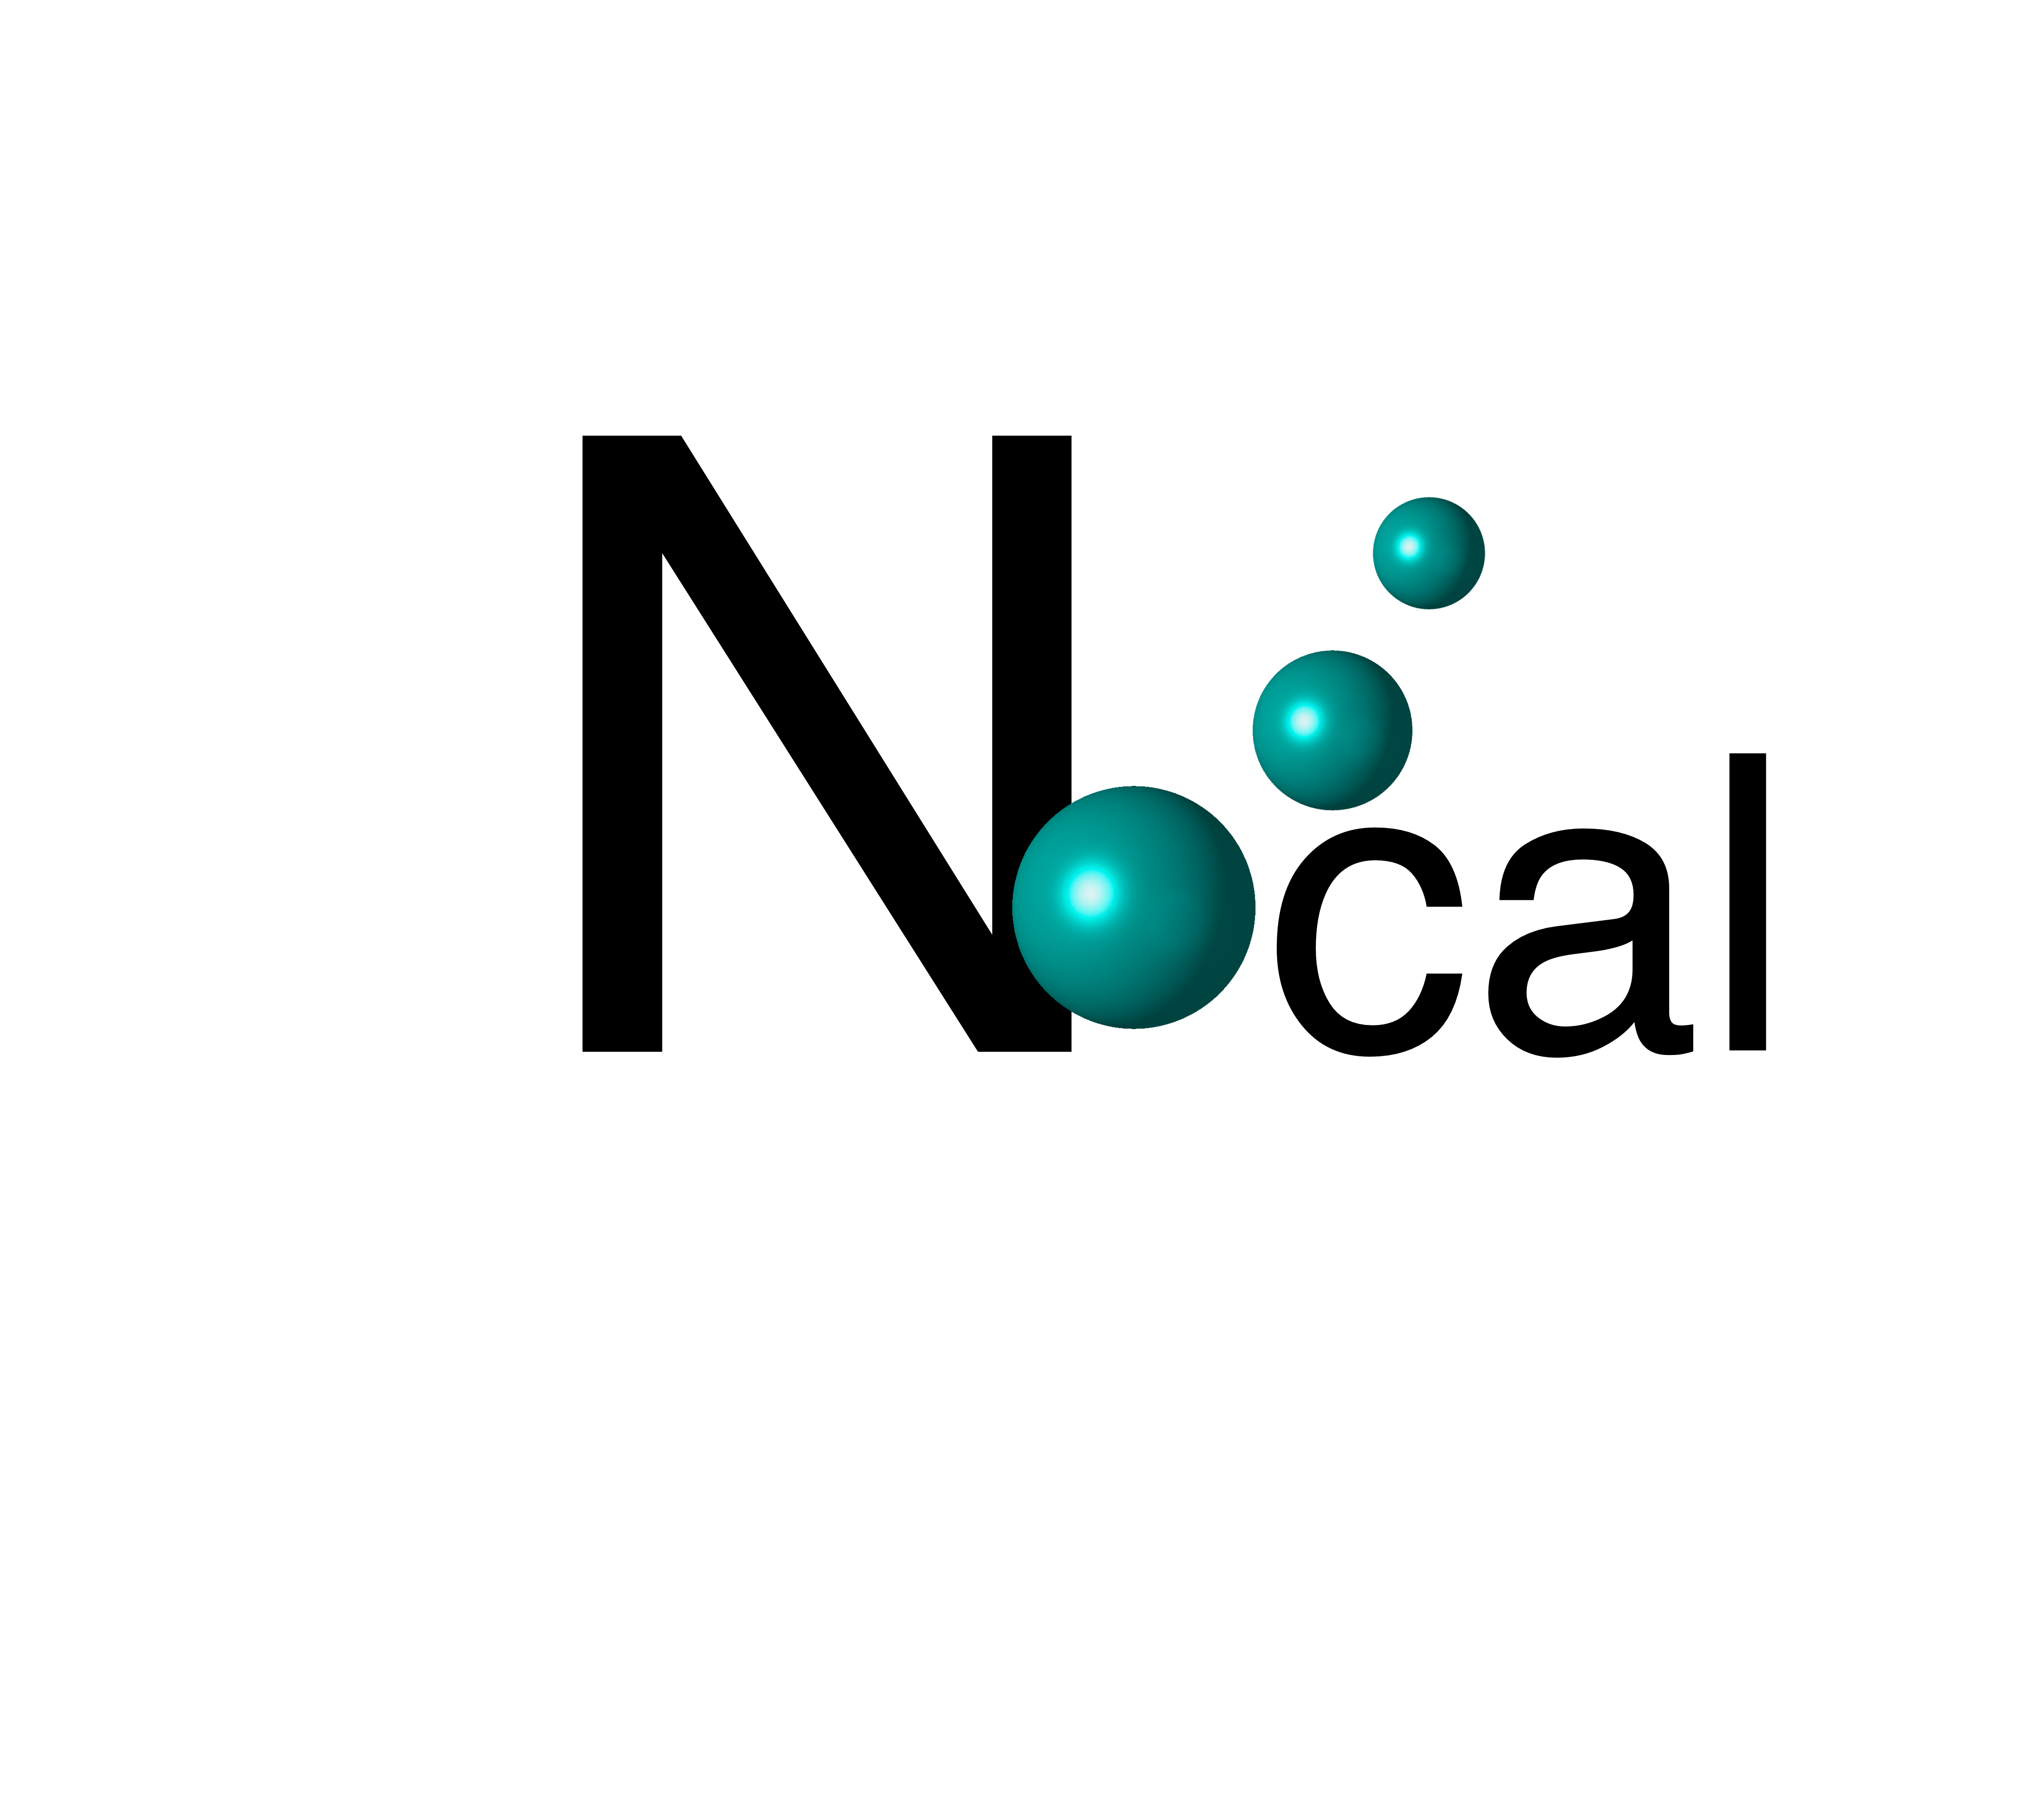
\includegraphics[trim={10cm 10cm 4cm 0cm},clip,  width=0.95\textwidth]{nocal.png}
\end{figure}
%%trim={<left> <lower> <right> <upper>}
%%
%%
{\centering  Version 0.1.0 \\
Developed by \\
John A. Moore, PhD \\
Caitlin Martinez \\
Ayushi Chandel  \\
$\hdots$ \\
Support\\
\url{john.a.moore@marquette.edu}\\
}
%%%%%%%%%%%%%%%%%%%%%%%%%%%%%%%%%%%%%%%
%%%%%%%%%%              INTRODUCTION       %%%%%%%%%%%%%%
%%%%%%%%%%%%%%%%%%%%%%%%%%%%%%%%%%%%%%%
\section{Introduction}
Nocal is python-based nonlocal pre/post processing software for nonlocal analysis of finite element analysis results. 
\section{Input Deck}
Nocal is controlled by a python dictionary where all the user inputs (i.e., \emph{cards}) are stored. This file must be called \inputDeckName. Each subsection describes a different card and the data type of each input is shown in italics next to the card
%%%%%%%%%%%%%%%%%%%%%%%%%%%%%%%%%%%%%%%
\subsection{deckName}
\emph{String} \\
If the user chooses to build the connectivity matrix from an Abaqus input deck, this is the name of the deck minus the .inp.\\
Example:\\
For an abaqus input deck named paraFipMesh\_11.inp \\
{$\tt{'deckName' : 'paraFipMesh\_11'}$}\\
Module Location\\
\begin{itemize}
  \item createAllNlElsetsInRegionParaNConf.py,
  \item getElemCent.py,
  \item nonlocalFIP.py,
  \item nonlocalFIPWeight.py
\end{itemize}
%%%%%%%%%%%%%%%%%%%%%%%%%%%%%%%%%%%%%%%
\subsection{dx}
\emph{Float} \\
The is the length of an edge of square nonlocal volume, for spherical nonconformal volumes Nocal will convert this value into a sphere with an equivalent volume to the cube with edges $dx$ \\
Example:\\
For $\Delta x = 0.215443469$ \\
$\tt{'dx' : 0.215443469}$
Module Location\\
\begin{itemize}
  \item createAllNlElsetsInRegionParaNConf.py,
\end{itemize}
%%%%%%%%%%%%%%%%%%%%%%%%%%%%%%%%%%%%%%%
\subsection{numProc}
\emph{Integer} \\
Number of processors to use when preprocessing nonlocal volumes \\
Example:\\
If you wanted to use 4 processors \\
$\tt{'numProc' : 4}$
Module Location\\
\begin{itemize}
  \item createAllNlElsetsInRegionParaNConf.py,
\end{itemize}
%%%%%%%%%%%%%%%%%%%%%%%%%%%%%%%%%%%%%%%
\subsection{isWeight}
\emph{boolean} \\
True if you want a weighted average over the nonlocal volume; False if you want a standard mean \\
The weighted average for a value $\Gamma$ is given by
%%%
%%%
\begin{equation}
\Gamma^{\textrm{nl}}(\pmb{x})  = \frac{1}{A(\pmb{x})}
\int_{\Omega}\phi(\pmb{x} - \pmb{y}) 
\Gamma^{\textrm{loc}}(\pmb{y}) d\Omega,
\label{eq:fipnl}
\end{equation}
%%%
%%%
where $\Gamma^{\textrm{loc}}$ and $\Gamma^{\textrm{nl}}$ are the local and nonlocal values of some finite element output $\Gamma$ respectively. The position where the nonlocal $\Gamma$ is calculated is $\pmb{x}$ and $\pmb{y}$ is positions around $\pmb{x}$ over which $\Gamma^{\textrm{loc}}$  is integrated. The nonlocal volume is $\Omega$, and  $\phi$ is a Gaussian distributed weighting function. The normalizing value of $A$ is given by 
%%%
%%%
\begin{equation}
A(\pmb{x}) = 
\int_{\Omega}\phi(\pmb{x} - \pmb{y}) 
 d\Omega,
\label{eq:a}
\end{equation}
%%%
%%%
and 
\begin{equation}
\phi(\pmb{x}) = 
\exp{(-||\pmb{x}||^2/l^2}),
\label{eq:phi}
\end{equation}
where $l$ is the nonlocal length scale.\\
Example:\\
if you want a weighted average \\
$\tt{'isWeight' : True}$
Module Location\\
\begin{itemize}
  \item runNonlocalFip.py
\end{itemize}
%%%%%%%%%%%%%%%%%%%%%%%%%%%%%%%%%%%%%%%
\subsection{resultsFileName}
\emph{String} \\
This is the name of the results file where you want to postprocess over the predetermined nonlocal values, you should include the extention (although what extension it is does not matter)\\
Example:\\
For a results file named paraFipMesh-FIP\_1\_11.txt\\
{$\tt{'resultsFileName' : 'paraFipMesh-FIP\_1\_11.txt'}$}\\
Module Location\\
\begin{itemize}
  \item nonlocalFIP.py,
  \item nonlocalFIPWeight.py
\end{itemize}
%%%%%%%%%%%%%%%%%%%%%%%%%%%%%%%%%%%%%%%
\subsection{L}
\emph{Float} \\
Length scale $l$ for \Eq \ref{eq:phi}, It is only used if isWeight=True\\
Example:\\
You want to weight over a region of $l=0.13365046175$\\
{$\tt{'L' : 0.13365046175}$}\\
Module Location\\
\begin{itemize}
  \item nonlocalFIPWeight.py
\end{itemize}
%%%%%%%%%%%%%%%%%%%%%%%%%%%%%%%%%%%%%%%
\subsection{isNonConf}
\emph{boolean} \\
Flag to tell if you should use conformal or nonconformal volumes
If you want conformal volumes isNonConf=True
If you want nonconformal volumes sNonConf=False \\
Example:\\
If you want conformal volumes \\
{$\tt{'isNonConf' : True}$}\\
Module Location\\
\begin{itemize}
  \item nonlocalFIP.py
\end{itemize}
%%%%%%%%%%%%%%%%%%%%%%%%%%%%%%%%%%%%%%%
\subsection{plotVolumes}
\emph{boolean} \\
Flag to tell if Nocal should produce plots of specific nonlocal volumes
If you want plots (stored in results) plotVolumes=True
If you do not want plots plotVolumes=False \\
Example:\\
If you want plots \\
{$\tt{'plotVolumes : True}$}\\
Module Location\\
\begin{itemize}
  \item plot.py
\end{itemize}
%%%%%%%%%%%%%%%%%%%%%%%%%%%%%%%%%%%%%%%
\subsection{vol2Plot}
\emph{float} or \emph{array}  \\
Only used if plotVolumes=True
This tells Nocal what number of volumes you want to plot. Note the plots are stored in the results directory and not actually pushed to the screen \\
Example:\\
If you want to plot volume 1, 3 and 50 \\
{$\tt{'vol2Plot' : [1,3,50]}$}\\
If you want to plot only volume 100 \\
{$\tt{'vol2Plot' : 100}$}\\
Module Location\\
\begin{itemize}
  \item plot.py
\end{itemize}
%%%%%%%%%%%%%%%%%%%%%%%%%%%%%%%%%%%%%%%
\subsection{runOnly}
\emph{string}   \\
This allows you to only run various parts of the preprocessing, plotting, or post processing. For example if you only want to plot some nonlocal volumes you can do this without having to re-determine all the nonlocal volumes and post processes, etc.
The options are
\begin{itemize}
  \item {\tt{getNlNodesElem}}, will only extract the nodes and elements from the mesh
    \item {\tt{getElemCent}}, will only extract the centroids on nodes and elements (which have to be already extracted from the mesh)
    \item {\tt{createVolume}}, will only create the nonlocal volumes 
      \item {\tt{plotNl}}, will only create plots and will not pre/post process anything
      \item {\tt{runNonlocalFip}}, will only post process the results
\end{itemize}
Example:\\
If you only want to plot and not pre/post process then \\
{$\tt{'runOnly': 'plotNl'}$}\\
If you want to run the whole code \\
{$\tt{'runOnly': 'none'}$}\\
Module Location\\
\begin{itemize}
  \item main.py
\end{itemize}
%%%%%%%%%%%%%%%%%%%%%%%%%%%%%%%%%%%%%%%
%%%%%%%%%%              RunningNocal       %%%%%%%%%%%%%%
%%%%%%%%%%%%%%%%%%%%%%%%%%%%%%%%%%%%%%%
\section{Running Nocal}
If all finite element input decks and all results files are in ./data (or .$\backslash$data) then run from your command line\\
{\tt{python \mainFileName}} \\
The results of any postprocessing are stored in ./results (or .$\backslash$results)
\end{document}